\documentclass[]{article}

\usepackage{amsmath}
\usepackage{bbm}
\usepackage{mathtools}
\usepackage{placeins}
\usepackage{nicefrac}

\usepackage[export]{adjustbox}

\usepackage{amsmath}
\DeclareMathOperator{\Tr}{Tr}
\DeclareMathOperator{\Var}{Var}
\DeclareMathOperator{\diff}{d}

%opening
\title{Disparity Map Estimation Using Graph Cuts}
\author{Marius Dufraisse}
\date{}

\begin{document}

\maketitle

\section*{Impact of the parameters}
\paragraph{Patch size.}
As the patch size increases results tend to be less noisy as small differences between the two image have less weight in the correlation computation. Increasing it too much on the other hand will yield a result with less details (see figure \ref{fig:win}).
\begin{figure}[h]
	\centering
	\begin{minipage}{0.24\linewidth}
		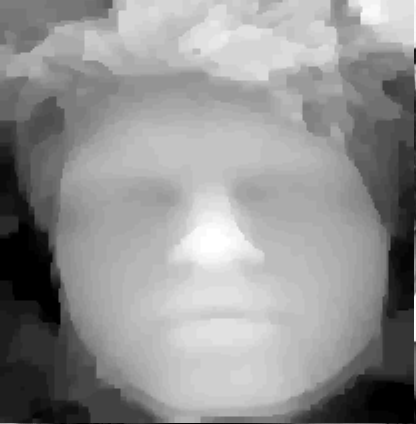
\includegraphics[width=\linewidth]{results/thierry_n3_l2.png}
	\end{minipage}\hfill
	\begin{minipage}{0.24\linewidth}
		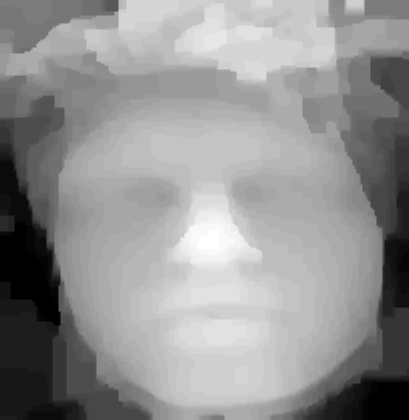
\includegraphics[width=\linewidth]{results/thierry_n5_l2.png}
	\end{minipage}\hfill
	\begin{minipage}{0.24\linewidth}
		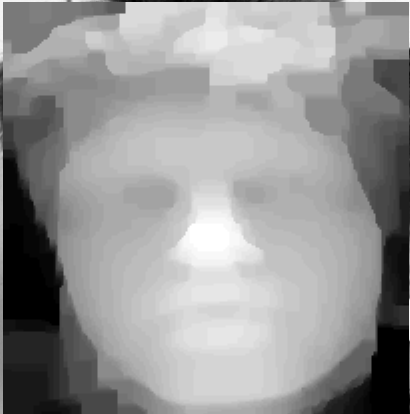
\includegraphics[width=\linewidth]{results/thierry_n7_l2.png}
	\end{minipage}\hfill
	\begin{minipage}{0.24\linewidth}
		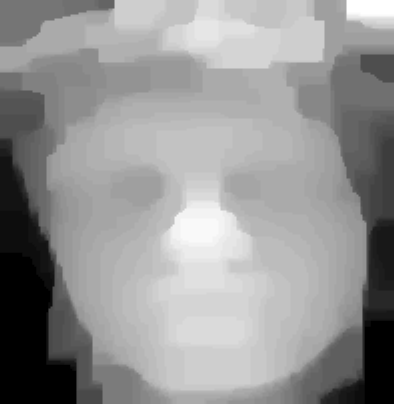
\includegraphics[width=\linewidth]{results/thierry_n12_l2.png}
	\end{minipage}
	\caption{Disparity map obtained for the provided images with patches of size 7, 11 , 15 and 25 and $\lambda = 2$.}
	\label{fig:win}
\end{figure}

\paragraph{Influence of $\lambda$.}
Small value of $\lambda$ will yield a noisy result as having lot of changes in disparity between neighbor pixels won't be penalized enough (see figure \ref{fig:lambda}). On the other hand if $\lambda$ is too large the optimal cut will have few disparity values.
\begin{figure}[h]
	\centering
	\begin{minipage}{0.24\linewidth}
		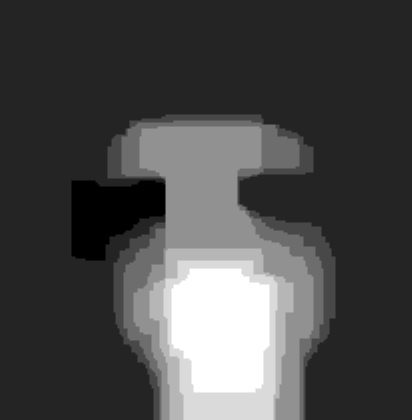
\includegraphics[width=\linewidth]{results/thierry_n3_l20.png}
	\end{minipage}\hfill
	\begin{minipage}{0.24\linewidth}
		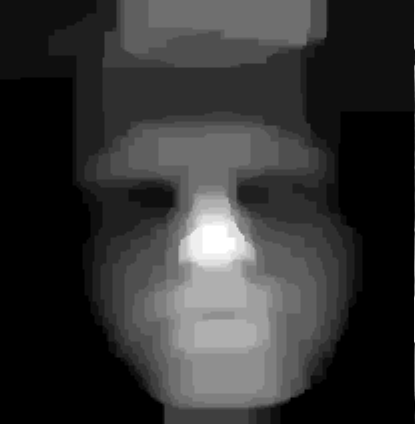
\includegraphics[width=\linewidth]{results/thierry_n3_l10.png}
	\end{minipage}\hfill
	\begin{minipage}{0.24\linewidth}
		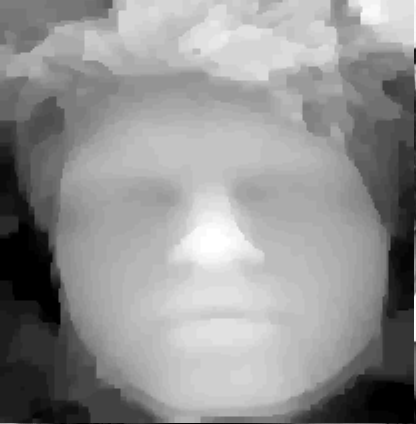
\includegraphics[width=\linewidth]{results/thierry_n3_l2.png}
	\end{minipage}\hfill
	\begin{minipage}{0.24\linewidth}
		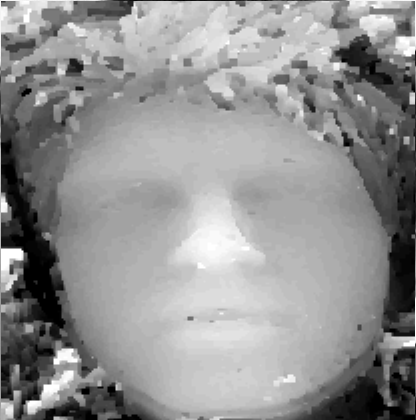
\includegraphics[width=\linewidth]{results/thierry_n3_l1.png}
	\end{minipage}
	\caption{Disparity map obtained for the provided images with $\lambda$ equal to 20, 10, 2 and 1 and patch size equal to 7.}
	\label{fig:lambda}
\end{figure}

Note that when setting $\lambda=0$ there is no interaction between neighbor pixel and thus we get a result similar to the NCC maximization method (see figure \ref{fig:lambda0}).
\begin{figure}[h]
	\centering
	\begin{minipage}{0.47\linewidth}
		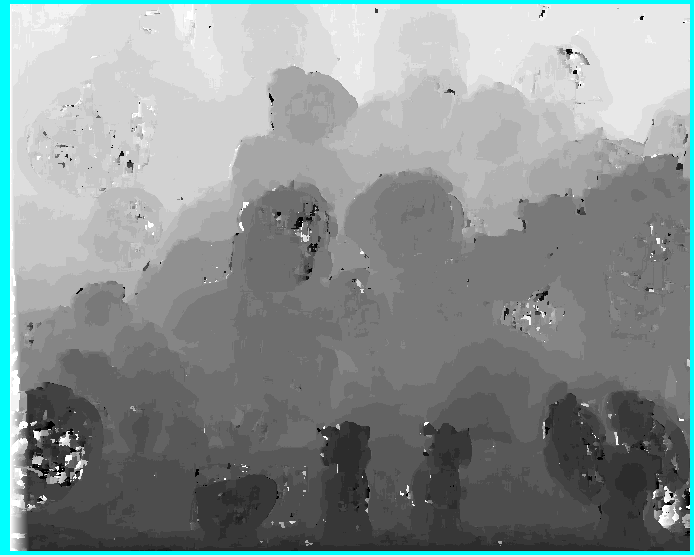
\includegraphics[width=\linewidth]{results/poup_full_monasse.png}
	\end{minipage}\hfill
	\begin{minipage}{0.47\linewidth}
		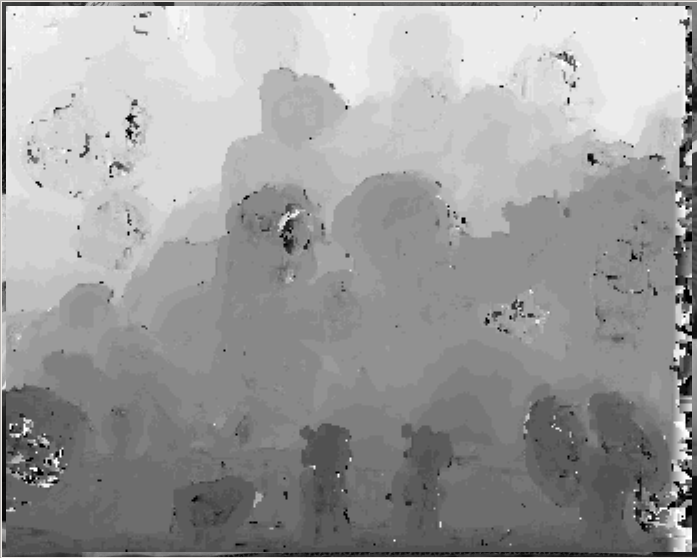
\includegraphics[width=\linewidth]{results/poup_l0_gc.png}
	\end{minipage}
	\caption{Left : result obtained by, for each pixel, taking the disparity that maximizes the NCC. Right : result obtained with the graph cut algorithm and $\lambda=0$. All other parameters (window size, disparity range) are equal except for the zoom used to speed up the computation in the graph cut algorithm. Input images are shown in figure \ref{fig:poupee}.}
	\label{fig:lambda0}
\end{figure}

\section*{Comparison with the region-growing method}
The graph-cut method is roughly two time faster than the region-growing one (26 seconds versus 56 seconds when using a zoom of 2 for the graph cut method and no cache of the average of patches in the region-growing method).

The graph-cut method yield result that are less noisy thanks to a global regularization (see figure \ref{fig:comp_poup}).
\begin{figure}[h]
	\centering
	\begin{minipage}{0.48\linewidth}
		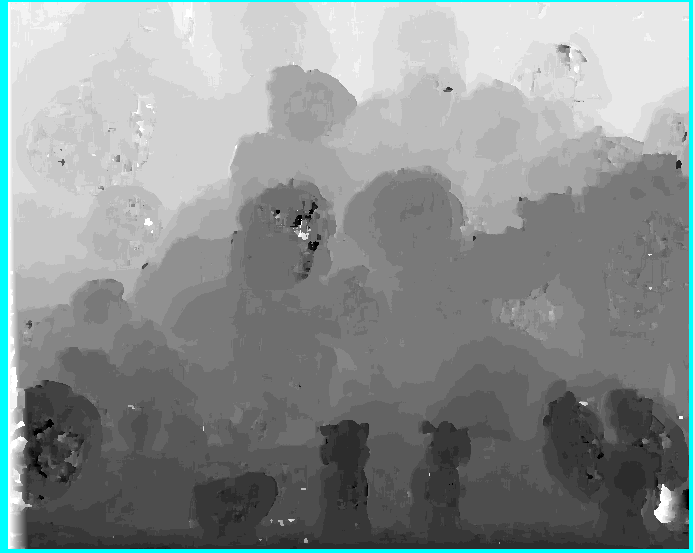
\includegraphics[width=\linewidth]{results/poup_monasse.png}
	\end{minipage}\hfill
	\begin{minipage}{0.48\linewidth}
		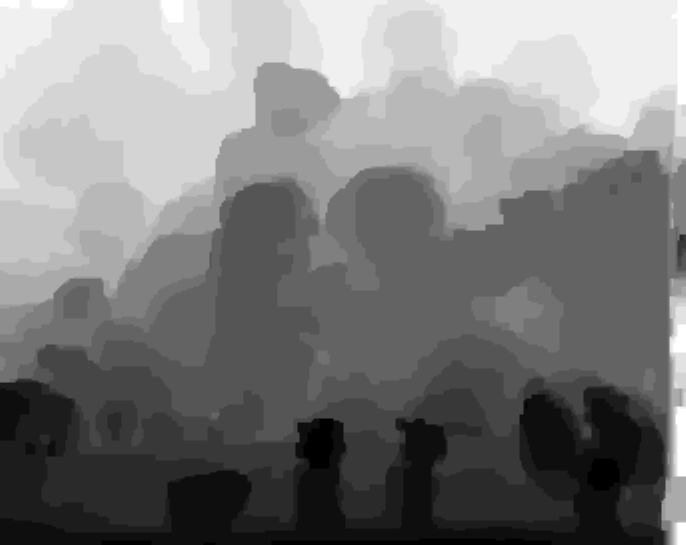
\includegraphics[width=\linewidth]{results/poup_same.png}
	\end{minipage}
	\caption{Left : results obtained with the region-growing method. Right: results obtained with the graph-cut method. Common parameters where taken to be equal. Input images are shown in figure \ref{fig:poupee}.}
	\label{fig:comp_poup}
\end{figure} 

\begin{figure}[h]
	\centering
	\begin{minipage}{0.47\linewidth}
		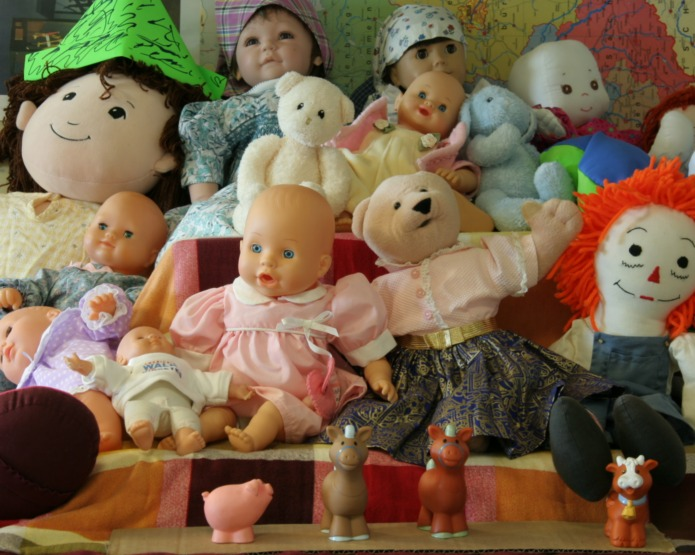
\includegraphics[width=\linewidth]{../Seeds/im1.jpg}	
	\end{minipage}\hfill
	\begin{minipage}{0.47\linewidth}
		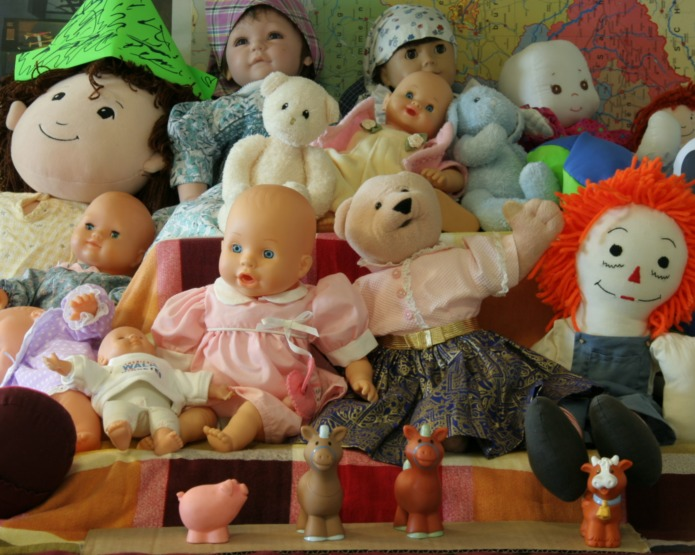
\includegraphics[width=\linewidth]{../Seeds/im2.jpg}
	\end{minipage}\hfill
	\caption{Pair of images used as input.}
	\label{fig:poupee}
\end{figure}

\end{document}
